% Chapter 2

\chapter{High-dimensional cosystoles and Cheeger constants}

\label{Chapter2}

When we want to determine whether a cochain is a cosystole or not (or in other words, to determine the cosystolic norm of a cochain) until now we only have the original definition of cosystolicity, which does not seem to be very useful. In this chapter we want to develop tools to get hands on this problem, especially by estimating the cosystolic norm in various situations and investigating the structure how cosystoles in certain simplicial complexes are arranged. Furthermore, at the end of this chaper we will develop some interesting statements about the shape of Cheeger cosystoles.

\section{Piercing sets and the cycle detection theorem}

The following definition is adopted from \cite{6}.

\begin{defi}
Let \(V\) be some set and \(\mathcal{F}\subseteq 2^V\) a family of finite subsets of \(V\). A subset \(P\subseteq V\) is called a \textbf{piercing set} of \(\mathcal{F}\) if we have \(P\cap F\neq\emptyset\) for all \(F\in\mathcal{F}\). The minimal cardinality of a piercing set of \(\mathcal{F}\), denoted by \(\tau(\mathcal{F})\), is called the \textbf{piercing number} of \(\mathcal{F}\).\\
For a \(v\in V\) and an \(F\in\mathcal{F}\) we say that \(F\) \textbf{is pierced by} \(v\), if \(v\in F\).
\end{defi}

\begin{expl}\label{example1}
Let \(V:=\left\{1,2,3,4,5\right\}\) and \(\mathcal{F}:=\left\{\{1,2\}\{2,3,4\},\{1,5\},\{2,4,5\}\right\}\), then we have \(\tau(\mathcal{F})=2\), since for example \(P:=\left\{2,5\right\}\) is a minimal piercing set of \(\mathcal{F}\).
\end{expl}

Later we will talk about piercing numbers and piercing sets of families of \(k\)-chains, which we define as follows:

\begin{defi}
Let \(X\) be a simplicial complex and \(\mathcal{F}\subseteq C_k(X)\) a family of \(k\)-chains. The \textbf{piercing sets} and the \textbf{piercing number} of \(\mathcal{F}\) are defined as the piercing sets and the piercing number of the family \(\left\{\supp(F)\text{ : }F\in\mathcal{F}\right\}\).
\end{defi}

In \cite{6} Kozlov stated the following useful method to bound the cosystolic norm of a cochain.

\begin{thm}[The cycle detection theorem]\label{theorem9}
Let \(X\) be a simplicial complex and \(\varphi\in C^k(X)\). Let now \(\mathcal{F}=\left\{\alpha_1,\ldots,\alpha_t\right\}\) be a family of \(k\)-cycles in \(C_k(X)\), such that \(\left\langle\varphi,\alpha_i\right\rangle=1\) for all \(1\leq i\leq t\), then we have:
\[
\|\varphi\|_{csy}\geq\tau(\mathcal{F})
\]
\begin{proof}
Let \(\psi\in C^{k-1}(X)\), then for any \(1\leq i\leq t\) we have:
\begin{align}
\langle\varphi+\delta^{k-1}(\psi),\alpha_i\rangle&=\langle\varphi,\alpha_i\rangle+\langle\delta^{k-1}(\psi),\alpha_i\rangle\notag\\
&=\langle\varphi,\alpha_i\rangle+\langle\psi,\partial_{k-1}(\alpha_i)\rangle\notag\\
&=\langle\varphi,\alpha_i\rangle+\langle\psi,0\rangle\notag\\
&=\langle\varphi,\alpha_i\rangle=1\notag
\end{align}
This means that we have \(\supp(\varphi+\delta^{k-1}(\psi))\cap \supp(\alpha_i)\neq\emptyset\) for all \(1\leq i\leq t\), so \(\supp(\varphi+\delta^{k-1}(\psi))\) is a piercing set of \(\mathcal{F}\) and we get:
\[
\|\varphi+\delta^{k-1}(\psi)\|=|\supp(\varphi+\delta^{k-1}(\psi))|\geq\tau(\mathcal{F})
\]
Since \(\psi\) was chosen arbitrarily we get the requested result.
\end{proof}
\end{thm}

The following corollary (a special case of the preceding theorem) was also stated by Kozlov in \cite{6}.

\begin{cor}\label{corollary1}
Let \(X\) be a simplicial complex and \(\varphi\in C^k(X)\).\\
Let now \(\mathcal{F}=\{\alpha_1,\ldots,\alpha_{\|\varphi\|}\}\) be a family of \(k\)-cycles in \(C_k(X)\), such that \(\left\langle\varphi,\alpha_i\right\rangle=1\) for all \(1\leq i\leq\|\varphi\|\) and \(\supp(\alpha_i)\cap \supp(\alpha_j)=\emptyset\) for all \(i\neq j\), then \(\varphi\) is a cosystole.
\begin{proof}
Since the supports of the cycles \(\alpha_1,\ldots,\alpha_{\|\varphi\|}\) are pairwise disjoint, we obviously have \(\tau(\mathcal{F})=\|\varphi\|\) and using the cycle detection theorem we are done.
\end{proof}
\end{cor}

\begin{expl}\label{example1a}
Consider the cochain
\[
\varphi=\left(\{1,2,4\}+\{2,5,6\}+\{3,4,6\}+\{2,4,6\}\right)^*\in C^2(\Delta^{[6]})
\]
(Figure \ref{figure1:Figure 1} illustrates how the support of this cochain can be imagined) and the family of cycles
\begin{align*}
\mathcal{F}=\{&\{1,2,3\}+\{1,2,4\}+\{1,4,3\}+\{2,4,3\},\\
&\{1,2,5\}+\{1,2,6\}+\{1,5,6\}+\{2,5,6\},\\
&\{3,4,5\}+\{3,4,6\}+\{3,5,6\}+\{4,5,6\},\\
&\{1,3,5\}+\{1,3,6\}+\{1,4,5\}+\{1,4,6\}+\\
&\{2,3,5\}+\{2,3,6\}+\{2,4,5\}+\{2,4,6\}\}\subset C_2(\Delta^{[6]}).
\end{align*}
It is easy to check that we have \(\left\langle\varphi,\alpha\right\rangle=1\) for all \(\alpha\in\mathcal{F}\) and \(\tau(\mathcal{F})=4\), so we get \(\|\varphi\|_{csy}\geq 4\) by the cycle detection theorem. We can immediately see, that \(\varphi\) is a cosystole, either by the fact, that we always have \(\|\varphi\|_{csy}\leq \|\varphi\|\), so in our case we have \(\|\varphi\|=4=\|\varphi\|_{csy}\), or by using the preceding corollary, since the supports of the cycles in \(\mathcal{F}\) are pairwise disjoint.\\
Note, that \(\varphi\) is even a Cheeger cosystole, since we have \(\|\varphi\|_{exp}=\frac{6}{4}\), so we know that for the case \(n=6\) and \(k=2\) the lower bound of the estimate \ref{equation1} is archieved, even if \(k+2\) does not devide \(n\).
\end{expl}

\begin{figure}[ht]
\centering
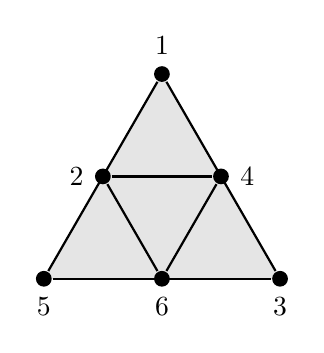
\begin{tikzpicture}[
       thick,
       acteur/.style={
         circle,
         fill=black,
         thick,
         inner sep=2pt,
         minimum size=0.2cm
       }
     ] 

	   \fill[fill=gray!20] (0,0)--(3,0)--(1.5,2.6);

       \node (a1) at (0,0) [acteur,label=below:5]{};
       \node (a2) at (3,0)[acteur,label=below:3]{}; 
       \node (a3) at (1.5,2.6) [acteur,label=above:1]{}; 
       \node (a4) at (0.75,1.3) [acteur,label=left:2]{}; 
       \node (a5) at (2.25,1.3) [acteur,label=right:4]{}; 
       \node (a6) at (1.5,0) [acteur,label=below:6]{};
  
       \draw (a1) -- (a2); 
       \draw (a2) -- (a3); 
       \draw (a1) -- (a3);
       
       \draw (a4) -- (a5);
       \draw (a5) -- (a6);
       \draw (a4) -- (a6);

\end{tikzpicture}
  \caption{The support of a $2$-Cheeger cosystole (The gray triangles represent the four $2$-simplices)}
  \label{figure1:Figure 1}
\end{figure}


To get the best possible results using the cycle detection theorem, the challenge is now for a certain cochain \(\varphi\) to find families of cycles such that they have a large piercing number and \(\varphi\) evaluates to \(1\) on every cycle. The following construction seems to be suited well to get hands on this problem.\\
For a cochain \(\varphi\in C^k(X)\) we define the following set of cycles:
\[
\mathcal{T}_{\varphi}:=\left\{\partial_k(\sigma)\text{ : }\sigma\in \supp(\delta^k(\varphi))\right\}
\]

\begin{prop}\label{proposition1a}
Let \(\varphi\in C^k(X)\), then we have:
\[
\|\varphi\|_{csy}\geq\tau(\mathcal{T}_{\varphi})
\]
\begin{proof}
By the definition of the coboundary map, we obviously have\\
\(\left\langle\varphi,\partial_k(\sigma)\right\rangle=1\) for all \(\partial_k(\sigma)\in\mathcal{T}_{\varphi}\) and so by the cycle detection theorem we are done.
\end{proof}
\end{prop}

Note that in many cases, even the equality \(\|\varphi\|_{csy}=\tau(\mathcal{T}_{\varphi})\) can be reached, but unfortunately this is not always true as the following example shows.

\begin{expl}\label{example1b}
Let \(\varphi\in C^2(\Delta^{[6]})\) be the cosystole from Example \ref{example1a}. We have:
\begin{align*}
\mathcal{T}_{\varphi}=\{&\{1,2,3\}+\{1,2,4\}+\{1,3,4\}+\{2,3,4\},\\
&\{1,2,4\}+\{1,2,5\}+\{1,4,5\}+\{2,4,5\},\\
&\{2,3,5\}+\{2,3,6\}+\{2,5,6\}+\{3,5,6\},\\
&\{1,2,5\}+\{1,2,6\}+\{1,5,6\}+\{2,5,6\},\\
&\{3,4,5\}+\{3,4,6\}+\{3,5,6\}+\{4,5,6\},\\
&\{1,3,4\}+\{1,3,6\}+\{1,4,6\}+\{3,4,6\}\}.
\end{align*}
It is easy to check that we get \(\tau(\mathcal{T}_{\varphi})=3\), but as shown in Example \ref{example1} we have \(\|\varphi\|_{csy}=4\).
\end{expl}

It seems to be very difficult to determine the piercing number of \(\mathcal{T}_{\varphi}\) explicitely, but the concept of piercing complexes might be useful on the way to solve this problem.

\section{Piercing complexes}

Let \(V\) be some set, \(\mathcal{F}\subset 2^V\) a family of subsets and \(P\) a piercing set of \(\mathcal{F}\). Then for any \(v\in V\) obviously \(P\cup\{v\}\) is also a piercing set of \(\mathcal{F}\). We can use this fact to construct a simplicial complex, which contains all information about the piercing sets for a given family of sets as follows:

\begin{defi}
Let \(V\) be a set and \(\mathcal{F}\subset 2^V\) a family of subsets. Then the \textbf{piercing complex} of \(\mathcal{F}\) is defined as:
\[
\Delta_{\mathcal{F}}:=\left\{V'\subseteq V,\text{ : }(V\setminus V')\cap F\neq\emptyset\text{ for all }F\in\mathcal{F}\right\}
\]
\end{defi}
So, \(\Delta_{\mathcal{F}}\) consists of all subsets of \(V\), such that their complements in \(V\) are piercing sets of \(\mathcal{F}\) and indeed, \(\Delta_{\mathcal{F}}\) defines a simplicial complex, since deleting an element from the complement of a piercing set is equivalent to adding an element to a piercing set, which preserves the condition of being a piercing set.\\

\begin{expl}
Let \(V\) be an arbitrary set and \(\mathcal{F}:=2^V\) its power set. Then the piercing complex \(\Delta_{\mathcal{F}}\) is empty, since even the complement of a single vertex \(v\in V\) is not a piercing set of \(\mathcal{F}\). More general for an arbitrary set \(V\) we have that \(\Delta_{\mathcal{F}}\) is empty if and only if \(\left\{v\right\}\in\mathcal{F}\), for all \(v\in V\).\\
On the other hand \(\Delta_{\mathcal{F}}\) is a complete simplex on \(\left|V\right|\) vertices if and only if \(\mathcal{F}\) is empty, since only in this case even the empty set is a piercing set of \(\mathcal{F}\).
\end{expl}

We can now reformulate the question of determining the piercing number \(\tau(\mathcal{F})\) by asking for the dimension of \(\Delta_{\mathcal{F}}\), since we have the equality:
\[
\tau(\mathcal{F})=\left| V\right|-\dim(\Delta_{\mathcal{F}})-1
\]
Since our main interest in this section will be to investigate the piercing complex of \(\mathcal{T}_{\varphi}\) for a given cochain \(\varphi\in C^k(X)\) (where \(X\) is some simplicial complex) we will use a shorter notation for this piercing complex and set \(\Delta_{\varphi}:=\Delta_{\mathcal{T}_{\varphi}}\). Then the preceding formula turns to:
\[
\tau(\mathcal{T}_{\varphi})=|X^{(k)}|-\dim(\Delta_{\varphi})-1
\]

% TO BE CHECKED !!!
%
%      |
%      |
%      v

%The first interesting observation about \(\Delta_{\varphi}\) is, that its top dimensional homology group vanishes in almost all cases.

%\begin{thm}
%Let \(n\geq k+3\) and \(\varphi\in C^k(X)\), then we have:
%\[
%H_{\dim(\Delta_{\varphi})}(\Delta_{\varphi})\cong 0
%\]
%\begin{proof}
%Let \(\sigma\in\Delta_{\varphi}\) be a maximal simplex (i.e. for all \(v\in X^{(k)}\setminus\sigma\), we have \(\sigma\cup\{v\}\notin\Delta_{\varphi}\)). Then \(X^{(k)}\setminus\sigma\) is a minimal piercing set of \(\mathcal{T}_{\varphi}\) (i.e. for all \(v\in X^{(k)}\setminus\sigma\) we have that \(X^{(k)}\setminus (\sigma\cup\{v\})\) is not a piercing set of \(\mathcal{T}_{\varphi}\). Now, let \(v\in\sigma\) and \(w\in X^{(k)}\setminus\sigma\), such that \((\sigma\setminus\{v\})\cup\{w\}\in\Delta_{\varphi}\), and let
%\[
%P_w:=\left\{c\in\mathcal{T}_{\varphi}\text{ : }w\in c\text{, }w'\notin c\text{ for all }w'\in X^{(k)}\setminus\sigma\text{, }w'\neq w\right\}
%\]
%be the set of cycles from \(\mathcal{T}_{\varphi}\), that were pierced by \(w\) but by no other elements from \(X^{(k)}\setminus\sigma\). Then \(\{v\}\) must be a piercing set of \(P_w\) but since \(v\) and \(w\) are distinct, we get \(\left|P_w\right|=1\).
%\end{proof}
%\end{thm}

%      ^
%      |
%      |
%      
% TO BE CHECKED !!!

\begin{thm}
Let \(X\) be a simplicial complex and \(\varphi\in C^k(X)\), then we have:
\[
\tilde{H}_i(\Delta_{\varphi})\cong 0\quad\text{for all }i\leq k-1
\]
\begin{proof}
Let \(\varphi\in C^k(X)\) be chosen arbitrarily. Then for all \(\sigma\in \supp(\delta^k(\varphi))\) we have \(\left|\supp(\partial_k(\sigma))\right|=k+2\). Therefore, for all \(S\subset X^{(k)}\) such that \(\left|S\right|\leq k+1\) we have that \(X^{(k)}\setminus S\) is a piercing set of \(\mathcal{T}_{\varphi}\). This just means, that \(\Delta_{\varphi}\) has a full \(k\)-skeleton, so we immediately get \(\tilde{H}_i(\Delta_{\varphi})\cong 0\) for all \(i\leq k-1\).
\end{proof}
\end{thm}

\begin{defi}
Let \(X\) be a simplicial complex on the vertex set \(V\). Then the simplicial complex
\[
X^{\lor}:=\left\{\sigma\subseteq V\text{ : }V\setminus\sigma\notin X\right\}
\]
is called the \textbf{Alexander dual} of \(X\).
\end{defi}

The following theorem can be found in \cite{8}.

\begin{thm}[The Alexander duality theorem]\label{theorem12}
Let \(X\) be a simplicial complex on \(n\) vertices and \(X^{\lor}\) its Alexander dual. Then we have:
\[
\tilde{H}_i(X)\cong\tilde{H}^{n-i-3}(X)
\]
\end{thm}

\begin{defi}
Let \(V\) be some set and \(\mathcal{F}\subseteq 2^V\) a family of subsets of \(V\). Then the simplicial complex
\[
\Delta\left[\mathcal{F}\right]:=\left\{\sigma\subseteq V\text{ : there exists an }F\in\mathcal{F}\text{ such that }\sigma\subseteq F\right\}
\]
is called the \textbf{induced complex} of \(\mathcal{F}\). 
\end{defi}

The following statement was developed in \cite{9}.

\begin{prop}\label{proposition13}
Let \(V\) be some set and \(\mathcal{F}\subseteq 2^V\) a family of subsets of \(V\). Then we have:
\[
\Delta\left[\bar{\mathcal{F}}\right]^{\lor}=\Delta_{\mathcal{F}}
\]
where we set \(\bar{\mathcal{F}}:=\left\{V\setminus F\text{ : }F\in\mathcal{F}\right\}\).
\begin{proof}


We have:
\begin{align*}
  & \sigma\in\Delta\left[\bar{\mathcal{F}}\right]^{\lor} \\
  \Longleftrightarrow \quad & V\setminus\sigma\notin\Delta\left[\bar{\mathcal{F}}\right] \\
  \Longleftrightarrow \quad & \nexists F\in\bar{\mathcal{F}}\text{ : }V\setminus\sigma\subseteq F \\
  \Longleftrightarrow \quad & \nexists F\in\bar{\mathcal{F}}\text{ : }(V\setminus\sigma)\cap(V\setminus F)=\emptyset \\
  \Longleftrightarrow \quad & \nexists F'\in\mathcal{F}\text{ : }(V\setminus\sigma)\cap F'=\emptyset \\
  \Longleftrightarrow \quad & V\setminus\sigma\text{ is a piercing set of }\mathcal{F} \\
  \Longleftrightarrow \quad & \sigma\in\Delta_{\mathcal{F}}
 \end{align*}
\end{proof}
\end{prop}

\begin{thm}
Let \(X\) be a finite simplicial complex and \(\varphi\in C^k(X)\), then we have:
\[
\tilde{H}_k(\Delta_{\varphi})\cong 0
\]
\begin{proof}
For all \(\partial_k(\sigma)\in\mathcal{T}_{\varphi}\) we have \(|\supp(\partial_k(\sigma))|=k+2\), so we get:
\[
\dim(\Delta[\bar{\mathcal{T}}_{\varphi}])=|X^{(k)}|-(k+2)-1=|X^{(k)}|-k-3
\]
Now, there exist no two simplices of dimension \(|X^{(k)}|-k-3\) in \(\Delta[\bar{\mathcal{T}}_{\varphi}]\),\\
such that they have a face in common, so we have:
\[
\tilde{H}_{|X^{(k)}|-k-3}(\Delta[\bar{\mathcal{T}}_{\varphi}])\cong 0
\]
By the Alexander duality theorem and Proposition \ref{proposition13} we get:
\[
\tilde{H}_k(\Delta_{\varphi})\cong\tilde{H}^k(\Delta_{\varphi})=\tilde{H}^{|X^{(k)}|-(|X^{(k)}|-k-3)-3}(\Delta_{\varphi})\cong 0,
\]
where the first isomorphy is true, because we consider homology / cohomology over a field and \(\Delta_{\varphi}\) is finite.
\end{proof}
\end{thm}

\section{Large cosystoles of a simplex}

In this section we focus our investigations onto the question, what is the largest norm, a cosystole can attain when the underlying simplicial complex is a complete simplex, where the first statement we make is still valid for general simplicial complexes.\\
Let us first introduce a simplicial complex which represents all the information about cosystoles we need.

\begin{defi}
Let \(X\) be a simplicial complex and \(1\leq k\leq \dim(X)\). Then the simplicial complex
\[
\mathcal{C}_k(X):=\left\{S\subseteq X^{(k)}\text{ : }\left(\sum\limits_{\sigma\in S}\sigma\right)^*\text{ is a cosystole}\right\}
\]
is called the \textbf{k-cosystolic complex} of \(X\).
\end{defi}

Obviously, \(\mathcal{C}_k(X)\) defines a simplicial complex, since removing a simplex from the support of a cosystole and considering the corresponding cochain again preserves cosystolicity.\\
Now, for any simplicial complex \(X\) and any \(1\leq k\leq \dim(X)\), we define the following number (the largest norm, a cosystole can attain):
\[
C_{max}(X,k):=\max\left\{\|\varphi\|_{csy}\text{ : }\varphi\in C^k(X)\right\}
\]
Note, that we have the relation \(\dim(\mathcal{C}_k(X))=C_{max}(X,k)-1\).\\
\\
For the sake of completeness we still define the following number of the smallest norm a non-cosystolic cochain can attain:
\[
C_{min}(X,k):=\min\left\{\|\varphi\|\text{ : }\varphi\in C^k(X)\text{, }\|\varphi\|>\|\varphi\|_{csy}\right\}
\]
Let us introduce to following family of cycles:
\[
\mathcal{T}_n^k:=\left\{\partial_k(\sigma)\text{ : }\sigma\in\binom{[n]}{k+2}\right\}
\]
Note, that if \(k\) is odd, then \(\mathcal{T}_n^k\) is exactly the same as \(\mathcal{T}_{\varphi}\) for the cochain \(\varphi=\left(\sum\limits_{\sigma\in\binom{[n]}{k+1}}\sigma\right)^*\).
We can use it now to determine a lower bound for the number \(C_{max}(\Delta^{[n]},k)\) if \(k\) is odd. 

\begin{prop}\label{proposition11}
Let \(k\) be odd, then we have:
\[
C_{max}(\Delta^{[n]},k)\geq \left\lceil\frac{\binom{n}{k+2}}{n-k-1}\right\rceil
\]
\begin{proof}
Since any simplex \(\sigma\in\binom{[n]}{k+1}\) intersects the support of exactly \(n-k-1\) cycles from \(\mathcal{T}_n^k\) if \(k\) is odd, any piercing set of \(\mathcal{T}_n^k\) must contain at least \(\left\lceil\frac{\binom{n}{k+2}}{n-k-1}\right\rceil\) elements and by Proposition \ref{proposition1a} we are done.
\end{proof}
\end{prop}

For the \(1\)-dimensional case we can even find a better estimate, since we are able to determine the piercing number of \(\mathcal{T}_n^1\) exactly. A more elementary proof of this estimate is given as Proposition \ref{proposition3}) in the following chapter, where we will even see, that equality can be reached, shown in Theorem \ref{theorem1}.

\begin{prop}\label{proposition112}
\(C_{max}(\Delta^{[n]},1)\geq\binom{n}{2}-\left\lfloor\frac{n^2}{4}\right\rfloor\)
\begin{proof}
Asking for the smallest piercing set of \(\mathcal{T}_n^1\) is equivalent to asking for the largest triangle-free graph (i.e. a graph on \(n\) vertices, containing as many edges as posssible, but no complete graph on \(3\) vertices as a subgraph) and taking the complement. Mantel's theorem (see \cite{7}) says, that a triangle-free graph on \(n\) vertices has at most \(\left\lfloor\frac{n^2}{4}\right\rfloor\) edges, so we immediately get:
\[
\tau(\mathcal{T}_n^1)=\binom{n}{2}-\left\lfloor\frac{n^2}{4}\right\rfloor
\]
and by Proposition \ref{proposition1a} we are done.
\end{proof}
\end{prop}

Unfortunately, determining the piercing number of \(\mathcal{T}_n^k\) for \(k\geq 2\), or equivalently, determining the largest \(k\)-uniform hypergraph on \(n\)-vertices, containing no complete \(k\)-uniform hypergraph on \(k+2\) vertices as a subhypergraph, seems to be very difficult (see \cite{7}), so we can not use the preceding procedure to say something about \(C_{max}(\Delta^{[n]},k)\) for larger \(k\)'s in general.\\
Nevertheless, we can exactly determine this number for the ultimate and the penultimate proper dimension as follows.

\begin{thm}\label{theorem7}
\(C_{max}(\Delta^{[n]},n-2)=1\), for all \(n\geq 3\)
\begin{proof}
Let \(\sigma\in\binom{[n]}{n-1}\) be chosen arbitrarily, \(\varphi:=\sigma^*\in C^{n-2}(\Delta^{[n]})\) and\\
\(\mathcal{F}:=\left\{\alpha\right\}\), where \(\alpha\) is the boundary of the single (\(n-1\))-dimensional simplex in \(\Delta^{[n]}\). Obviously, we have \(\left\langle\varphi,\alpha\right\rangle=1\), since \(\supp(\varphi)\cap \supp(\alpha)=\supp(\varphi)\) and \(\tau(\mathcal{F})=1\), so by the cycle detection theorem we have \(\|\varphi\|_{csy}\geq 1\).\\
Now, let \(\sigma_1,\sigma_2\in\binom{[n]}{n-1}\) be chosen arbitrarily again (\(\sigma_1\neq\sigma_2\)) and \(c:=\sigma_1\cap\sigma_2\). Then we have \(\delta^{n-3}(c^*)+\sigma_1^*+\sigma_2^*=0\), so there exists no (\(n-2\))-cosystole attaining norm \(2\) and we are done.
\end{proof}
\end{thm}

\begin{lem}\label{lemma12}
Let \(n\geq 4\), then we have:
\[
\tau(\mathcal{T}_n^{n-3})=\left\lceil\frac{n}{2}\right\rceil
\]
\begin{proof}
For each \(\sigma\in\binom{[n]}{n-2}\) there exist exactly two cycles \(\alpha_1,\alpha_2\in\mathcal{T}_n^{n-3}\)\\
(\(\alpha_1\neq\alpha_2\)), such that \(\sigma\in \supp(\alpha_1)\cap \supp(\alpha_2)\), so the largest possible number of cycles from \(\mathcal{T}_n^{n-3}\) that can be pierced by one simplex is two. Furthermore, we have \(\left|\mathcal{T}_n^{n-3}\right|=\binom{n}{n-1}=n\), so we get \(\tau(\mathcal{T}_n^{n-3})\geq\left\lceil\frac{n}{2}\right\rceil\).\\
On the other hand, for all \(\alpha_1,\alpha_2\in\mathcal{T}_n^{n-3}\) there exists a \(\sigma\in\binom{[n]}{n-2}\), such that\\
\(\sigma\in \supp(\alpha_1)\cap \supp(\alpha_2)\), so we get \(\tau(\mathcal{T}_n^{n-3})\leq\left\lceil\frac{n}{2}\right\rceil\).
\end{proof}
\end{lem}

\begin{lem}\label{lemma13}
Let \(S\subset\binom{[n]}{n-2}\), such that \(\left|S\right|\geq\left\lfloor\frac{n}{2}\right\rfloor+1\), then there exist \(\sigma,\sigma'\in S\) \((\sigma\neq\sigma')\), such that \(\left|\sigma\cap\sigma'\right|=n-3\).
\begin{proof}
For \(\sigma,\sigma'\in\binom{[n]}{n-2}\) the condition \(\left|\sigma\cap\sigma'\right|<n-3\) is equivalent to the condition \(([n]\setminus\sigma)\cap([n]\setminus\sigma')=\emptyset\). Since we obviously have \(\left|[n]\setminus\sigma\right|=2\) for all \(\sigma\in\binom{[n]}{n-2}\) we can find at most \(\left\lfloor\frac{n}{2}\right\rfloor\) simplices \(\sigma_1,\ldots,\sigma_{\left\lfloor\frac{n}{2}\right\rfloor}\in\binom{[n]}{n-2}\), such that the sets \([n]\setminus\sigma_1,\ldots,[n]\setminus\sigma_{\left\lfloor\frac{n}{2}\right\rfloor}\) are pairwise disjoint and we are done.
\end{proof}
\end{lem}

\begin{thm}
\(C_{max}(\Delta^{[n]},n-3)=\left\lfloor\frac{n}{2}\right\rfloor\), for all \(n\geq 4\)
\begin{proof}
Let \(S\subset\binom{[n]}{n-2}\) be a minimal piercing set of \(\mathcal{T}_n^{n-3}\) as constructed in the proof of Lemma \ref{lemma12} and \(\varphi:=S^*\in C^{n-3}(\Delta^{[n]})\).\\
If \(n\) is even, then \(n-3\) is odd, so apply Proposition \ref{proposition1a} and Lemma \ref{lemma12} and we get:
\[
C_{max}(\Delta^{[n]},n-3)\geq\tau(\mathcal{T}_n^{n-3})=\frac{n}{2}
\]
If \(n\) is odd then by the construction of \(\varphi\) there exists exactly one \(\alpha'\in\mathcal{T}_n^{n-3}\), such that \(\left\langle\varphi,\alpha'\right\rangle=0\), since \(\left|\supp(\alpha')\cap \supp(\varphi)\right|=2\). Set \(\mathcal{F}:=\mathcal{T}_n^{n-3}\setminus\alpha'\), then we have \(\left\langle\varphi,\alpha\right\rangle=1\) for all \(\alpha\in\mathcal{F}\) and \(\tau(\mathcal{F})\geq\tau(\mathcal{T}_n^{n-3})-1=\left\lceil\frac{n}{2}\right\rceil-1=\left\lfloor\frac{n}{2}\right\rfloor\) by Lemma \ref{lemma12}, so by the cycle detection theorem we get \(C_{max}(\Delta^{[n]},n-3)\geq\left\lfloor\frac{n}{2}\right\rfloor\). One the other hand let \(\varphi\in C^{n-3}(\Delta^{[n]})\), such that \(\|\varphi\|=\left\lfloor\frac{n}{2}\right\rfloor+1\), then by Lemma \ref{lemma13} there exist \(\sigma_1,\sigma_2\in \supp(\varphi)\), such that \(\left|\sigma_1\cap\sigma_2\right|=n-3\). Now set \(\psi:=(\sigma_1\cap\sigma_2)^*\in C^{n-4}(\Delta^{[n]})\), then we have \(\|\delta^{n-4}(\psi)\|=3\) and \(\left|\supp(\delta^{n-4}(\psi))\cap \supp(\varphi)\right|\geq 2\). Thus, we have \(\|\delta^{n-4}(\psi)+\varphi\|\leq\|\varphi\|-1\) and \(\varphi\) can not be a cosystole, so we get \(C_{max}(\Delta^{[n]},n-3)\leq\left\lfloor\frac{n}{2}\right\rfloor\) and we are done.
\end{proof}
\end{thm}

\section{Embeddings of cosystoles}

When searching for cosystoles another approach is to consider cochains, which are already proven to be cosystolic and try to, roughly speaking, change or extend them to create new cosystoles. The most obvious way to do this is just to add a vertex to the underlying simplex by the embedding:

\begin{align*}
i_n^k\text{ : }C^k(\Delta^{[n]})&\longrightarrow C^k(\Delta^{[n+1]})\notag\\
\varphi&\longmapsto\left(\sum\limits_{\sigma\in\supp(\varphi)}\sigma\right)^*
\end{align*}

The first observation is, that cosystolicity is preserved by this embedding.

\begin{lem}\label{lemma132}
Let \(\varphi\in C^k(\Delta^{[n]})\) be a cosystole, then \(i_n^k(\varphi)\in C^k(\Delta^{[n+1]})\) is a cosystole.
\begin{proof}
Let \(\phi\in C^{k-1}(\Delta^{[n+1]})\) and consider the partition \(\supp(\phi)=C_1\cup C_2\) with\\
\(C_1:=\left\{\sigma\in\supp(\phi)\text{ : }n+1\in\sigma\right\}\) and \(C_2=\left\{\sigma\in\supp(\phi)\text{ : }n+1\notin\sigma\right\}\). Now set \(\phi_1:=C_1^*\) and \(\phi_2:=C_2^*\), then we have
\[
\delta^{k-1}(\phi)+i_n^k(\varphi)=\delta^{k-1}(\phi_1)+\delta^{k-1}(\phi_2)+i_n^k(\varphi),
\]
but \(\|\delta^{k-1}(\phi_2)+i_n^k(\varphi)\|\geq\|i_n^k(\varphi)\|\) holds by assumption and\\
\(\supp(\delta^{k-1}(\phi_1))\cap\supp(i_n^k(\varphi))=\emptyset\) holds by the construction of \(\psi_1\), so we get
\[
\|\delta^{k-1}(\phi)+i_n^k(\varphi)\|\geq\|i_n^k(\varphi)\|
\]
and we are done.
\end{proof}
\end{lem}

Furthermore, if \(\varphi\) is a cosystole, the coboundary expansions of \(\varphi\) and \(i_n^k(\varphi)\) are related as follows.

\begin{prop}\label{proposition113}
Let \(\varphi\in C^k(\Delta^{[n]})\) be a cosystole, then we have:
\[
\|i_n^k(\varphi)\|_{exp}=\|\varphi\|_{exp}+1
\]
\begin{proof}
By Lemma \ref{lemma132} we know that \(i_n^k(\varphi)\) is a cosystole and we have \(\|\delta^k(i_n^k(\varphi))\|=\|\delta^k(\varphi)\|+\|\varphi\|\), since for every simplex \(\sigma\) in the support of \(\varphi\), we get the additional simplex \((\sigma,n+1)\) in the support of \(\delta^k(i_n^k(\varphi))\). Hence, we have:
\[
\|i_n^k(\varphi)\|_{exp}=\frac{\|\delta^k(\varphi)\|+\|\varphi\|}{\|\varphi\|}=\|\varphi\|_{exp}+1
\]
\end{proof}
\end{prop}

\section{Multi-suspensions}

Another approach to create new cosystoles is to not only include a cochain into a higher dimensional simplex, but even increase the dimension of the cochain's support, which can be realized by the so called multi-suspensions.

\begin{defi}
Let \(0\leq k\leq n-1\) and \(d\geq 1\), then we call
\begin{align}
\sus_{n,k}^d:C^k(\Delta^{[n]})&\longrightarrow C^{k+1}(\Delta^{[n+d]})\notag\\
\varphi&\longmapsto\left(\sum\limits_{m=n+1}^d\left(\sum\limits_{\sigma\in \supp(\varphi)}(\sigma,m)\right)\right)^*\notag
\end{align}
the \textbf{suspension map of degree d}. Note, that \(\sus_{n,k}^d\) can also be easily defined on chain complexes by:
\begin{align}
\sus_{n,k}^d:C_k(\Delta^{[n]})&\longrightarrow C_{k+1}(\Delta^{[n+d]})\notag\\
c&\longmapsto\sum\limits_{\sigma\in \supp(\sus_{n,k}^d(c^*))}\sigma\notag
\end{align}
\end{defi}

\begin{lem}\label{lemma11}
Let \(\varphi\in C^k(\Delta^{[n]})\) and \(\mathcal{F}=\left\{\alpha_1,\ldots,\alpha_t\right\}\subset C_k(\Delta^{[n]})\) be a family of cycles, such that \(\left\langle\varphi,\alpha_i\right\rangle=1\) for all \(i=1,\ldots,t\). Then for each \(d\geq 1\) there exists a family of cycles \(\mathcal{F}'=\left\{\alpha_{1,1}',\ldots,\alpha_{t,d}'\right\}\subset C_{k+1}(\Delta^{[n+d]})\), such that \(\left\langle \sus_{n,k}^d(\varphi),\alpha_{i,j}'\right\rangle=1\) for all \(i=1,\ldots,t\) and \(j=1,\ldots,d\).
\begin{proof}
For each \(i=1,\ldots,t\) let \(c_i\in C_{k+1}(\Delta^{[n]})\), such that \(\partial_k(c_i)=\alpha_i\). For a simplex \(\sigma\in\binom{[n]}{k+1}\) and some \(n+1\leq j\leq n+d\) we have
\[
\partial_k\left((\sigma,j)\right)=\left(\sum\limits_{\sigma'\in \supp(\partial_{k-1}(\sigma))}(\sigma',j)\right)+\sigma
\]
So, we get
\begin{align*}
\partial_k\left(\sum\limits_{\sigma\in \supp(\alpha_i)}(\sigma,j)\right)&=\sum\limits_{\sigma\in \supp(\alpha_i)}\partial_k\left((\sigma,j)\right)\\
&=\sum\limits_{\sigma\in \supp(\alpha_i)}\left(\left(\sum\limits_{\sigma'\in \supp(\partial_{k-1}(\sigma))}(\sigma',j)\right)+\sigma\right)\\
&=\left(\sum\limits_{\sigma\in \supp(\alpha_i)}\quad\sum\limits_{\sigma'\in \supp(\partial_{k-1}(\sigma))}(\sigma',j)\right)+\alpha_i\\
&=0+\alpha_i\\
&=\alpha_i,
\end{align*}
since we have
\[
\sum\limits_{\sigma\in \supp(\alpha_i)}\quad\sum\limits_{\sigma'\in \supp(\partial_{k-1}(\sigma))}\sigma'=\partial_{k-1}(\alpha_i)=0
\]
for all \(i=1,\ldots,t\).\\
Thus, for all \(i=1,\ldots,t\) and \(j=n+1,\ldots,n+d\),
\[
\alpha_{i,j}:=\sum\limits_{\sigma\in \supp(\alpha_i)}(\sigma,j)+c_i
\]
defines a cycle, since we have
\[
\partial_k\left(\sum\limits_{\sigma\in \supp(\alpha_i)}(\sigma,j)+c_i\right)=\alpha_i+\alpha_i=0.
\]
Furthermore, we get
\begin{align}
\left\langle \sus_{n,k}^d(\varphi),\alpha_{i,j}\right\rangle&=\left\langle\left(\sum\limits_{m=n+1}^d\left(\sum\limits_{\sigma\in \supp(\varphi)}(\sigma,m)\right)\right)^*,\sum\limits_{\sigma\in \supp(\alpha_i)}(\sigma,j)+c_i\right\rangle\notag\\
&=\left\langle\left(\sum\limits_{\sigma\in \supp(\varphi)}(\sigma,j)\right)^*,\sum\limits_{\sigma\in \supp(\alpha_i)}(\sigma,j)+c_i\right\rangle\notag\\
&=1,\notag
\end{align}
since we have
\[\left\langle\varphi,\alpha_i\right\rangle=\left\langle\left(\sum\limits_{\sigma\in \supp(\varphi)}\sigma\right)^*,\sum\limits_{\sigma\in \supp(\alpha_i)}\sigma\right\rangle=1.
\]
\end{proof}
\end{lem}

\begin{defi}
Let \(V\) be some set, \(\mathcal{F}\subseteq 2^V\) a family of subsets of \(V\) and \(P=(p_1,\ldots,p_m)\) a finite ordered piercing set of \(\mathcal{F}\). Furthermore, set \(P_0:=\emptyset\) and for each \(i=1,\ldots,m\) set \(P_i:=\left\{F\in\mathcal{F}\text{ : }F\cap\{p_i\}\neq\emptyset\right\}\setminus P_{i-1}\). Then the tuple \(\lambda_P:=(|P_1|,\ldots,|P_m|)\) is called the \textbf{piercing sequence} of \(P\).
\end{defi}

\begin{prop}
Let \(\varphi\in C^k(\Delta^{[n]})\) and \(\mathcal{F}=\left\{\alpha_1,\ldots,\alpha_t\right\}\subset C_k(\Delta^{[n]})\) be a family of cycles, such that \(\left\langle\varphi,\alpha_i\right\rangle=1\), for all \(i=1,\ldots,t\) and \(P=(p_1,\ldots,p_m)\) an ordered piercing set of \(\mathcal{F}\), such that \(\tau(\mathcal{F})=m\). Then for any \(d\geq 1\) we have:
\[
\|\sus_{n,k}^d(\varphi)\|_{csy}\geq d\cdot\left|\left\{\beta\in\lambda_P\text{ : }\beta\geq d\right\}\right|+\sum\limits_{\beta\in\lambda_P\text{, }\beta<d}\beta
\]
\begin{proof}

\end{proof}
\end{prop}

\begin{prop}
Let \(\varphi\in C^k(\Delta^{[n]})\) and \(d\geq 1\), then we have:
\[
\|\delta^{k+1}(\sus_{n,k}^d(\varphi))\|=d\cdot\|\delta^k(\varphi)\|
\]
\begin{proof}

\end{proof}
\end{prop}

\section{On Cheeger cosystoles when k+2 does not devide n}

In \cite{4} and \cite{6} Meshulam and Kozlov gave examples of Cheeger cosystoles in \(C^k(\Delta^{[n]})\) when \(k+2\) devides \(n\). Recall, that is this case the Cheeger constant is explicitly determined by \(h_k(\Delta^{[n]})=\frac{n}{k+2}\). For the case when \(k+2\) does not devide \(n\), we can still explore some interesting properties about Cheeger cosystoles in terms of their norm.

\begin{prop}
Let \(\varphi\in C^k(\Delta^{[n]})\) be a Cheeger cosystole, such that \(\|\varphi\|_{exp}=\frac{n}{k+2}\), then \(k+2\) divides \(n\) or \(k+2\) devides \(\|\varphi\|\).
\begin{proof}
We have \(\|\delta^k(\varphi)\|=\frac{n\|\varphi\|}{k+2}\), since
\[
\frac{\|\delta^k(\varphi)\|}{\|\varphi\|}=\|\varphi\|_{exp}=\frac{n}{k+2}=\frac{n\|\varphi\|}{(k+2)\|\varphi\|}=\frac{\frac{n\|\varphi\|}{k+2}}{\|\varphi\|},
\]
but \(\|\delta^k(\varphi)\|\) is a natural number, so \(k+2\) must devide \(n\) or \(\|\varphi\|\).
\end{proof}
\end{prop}
